\documentclass[10pt]{article}
\usepackage[margin=0.8in]{geometry}
\usepackage{graphicx}
\usepackage{multicol}
\usepackage{float}
\graphicspath{{./images/}}
\usepackage{etoolbox}
\usepackage{longtable}
\usepackage{titlesec}
\setlength{\parskip}{0pt}

\begin{document}
\begin{figure}[H]
	\centering
	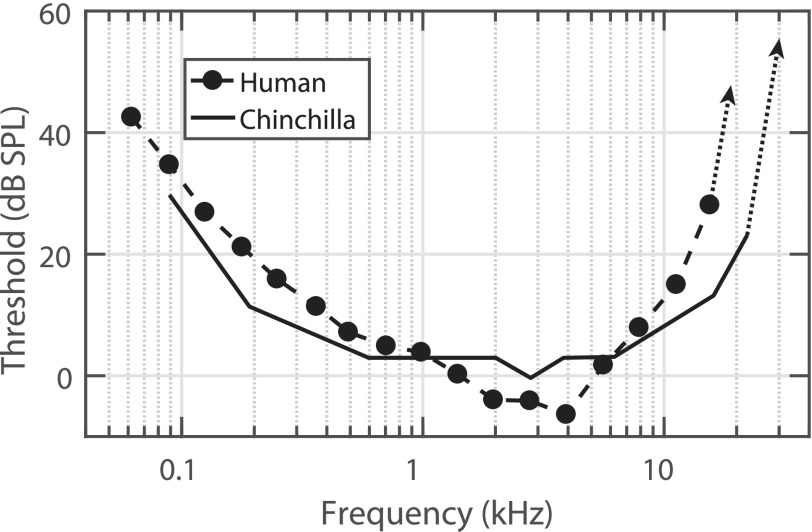
\includegraphics[height=2in]{response}
	\caption{Vestibulocochlear response in humans and chinchillas}
	\label{response}
\end{figure}
\begin{figure}[H]
	\centering
	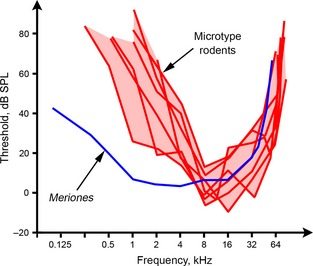
\includegraphics[height=2in]{response2}
	\caption{Vestibular response of chinchillas in comparison to other rodents}
	\label{response2}
\end{figure}

\begin{figure}[H]
	\centering
	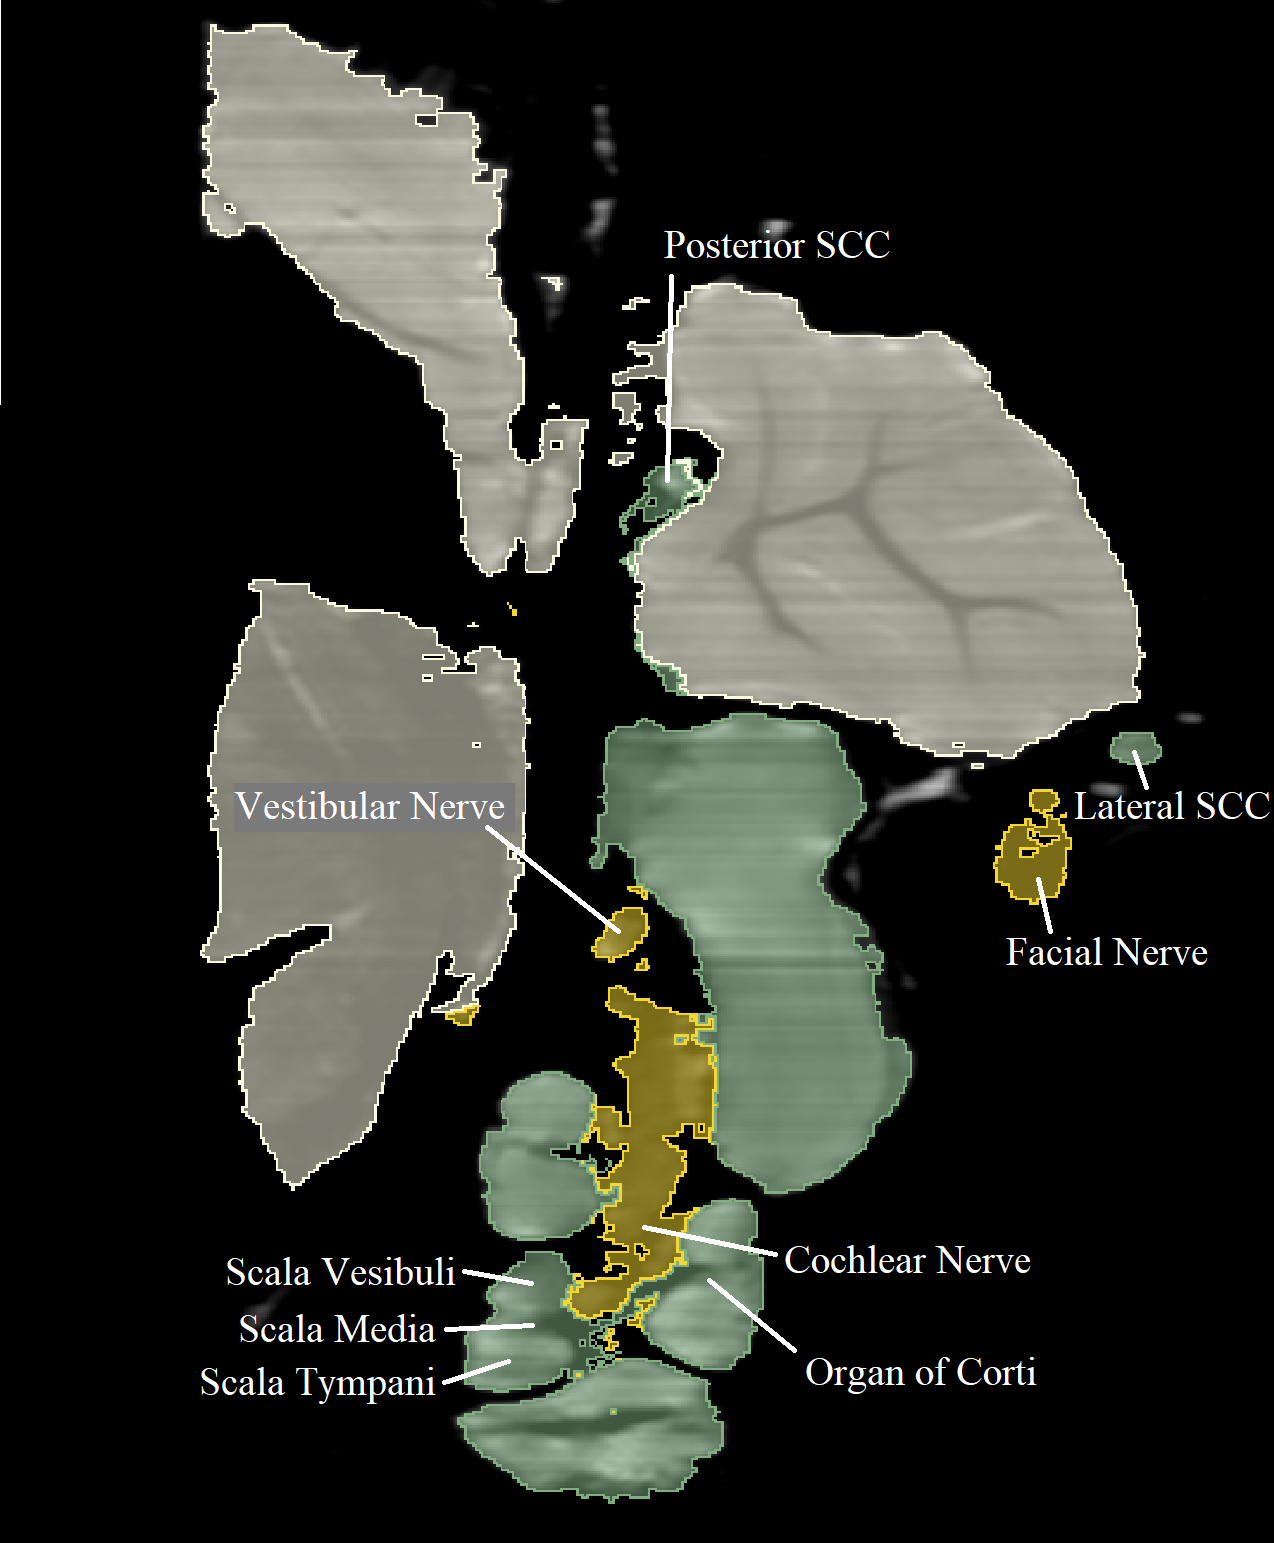
\includegraphics[scale=0.5]{segment2}
	\caption{The bony labyrinth of the cochlea and vestibular system is highlighted in green, nervous tissue in yellow, and brain tissue in white}
	\label{segment2}
\end{figure}

\begin{figure}[H]
	\centering
	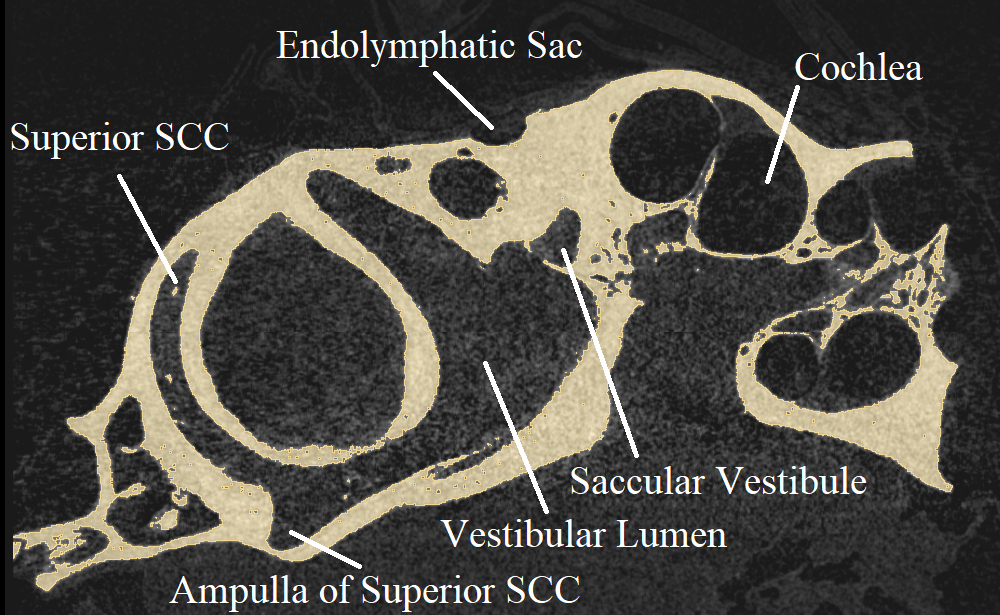
\includegraphics[width=\linewidth]{ctsegment}
	\caption{Osseous tissue is highlighted in white}
	\label{ctsegment}
\end{figure}

\begin{figure}[H]
	\centering
	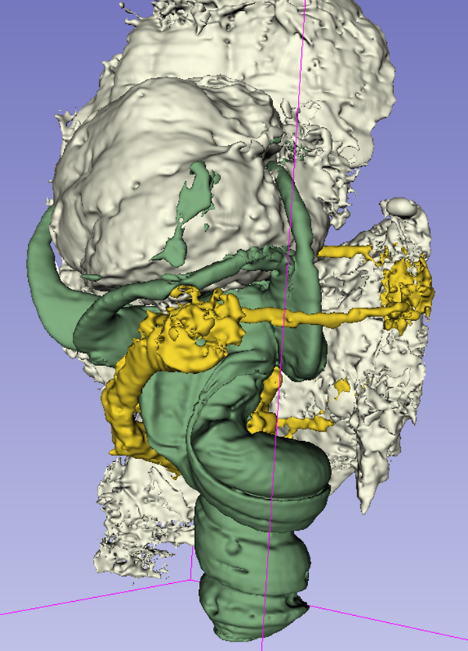
\includegraphics[height=3in]{pointcloud}
	\caption{Point cloud rendered in 3D Slicer with the bony labyrinth in green, brain tissue in white, and nervous tissue in yellow}
	\label{pc}
\end{figure}

\begin{figure}[H]
	\centering
	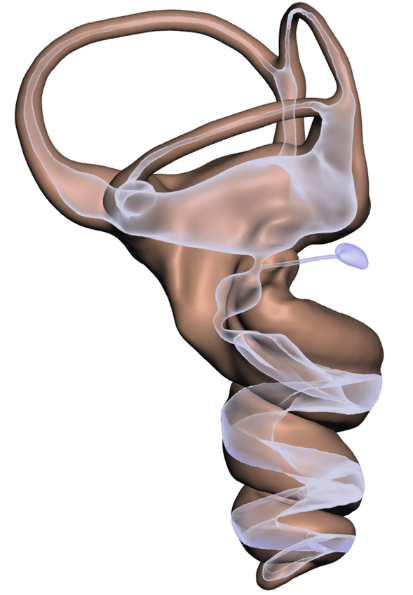
\includegraphics[height=3in]{translucentML}
	\caption{The membranous labyrinth is shown in clear within the tan bony labyrinth}
	\label{clearML}
\end{figure} 

\begin{figure}[H]
	\centering
	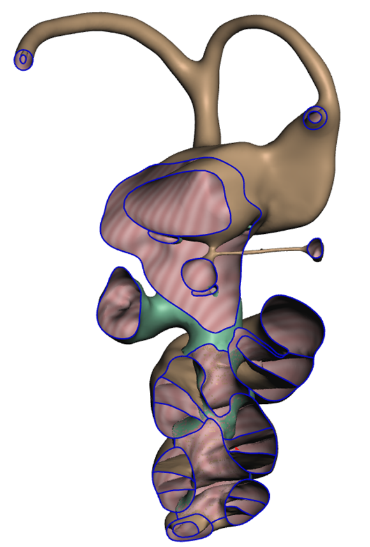
\includegraphics[height=3in]{bullacx}
	\caption{cx}
	\label{cx}
\end{figure}

\begin{figure}[H]
	\centering
	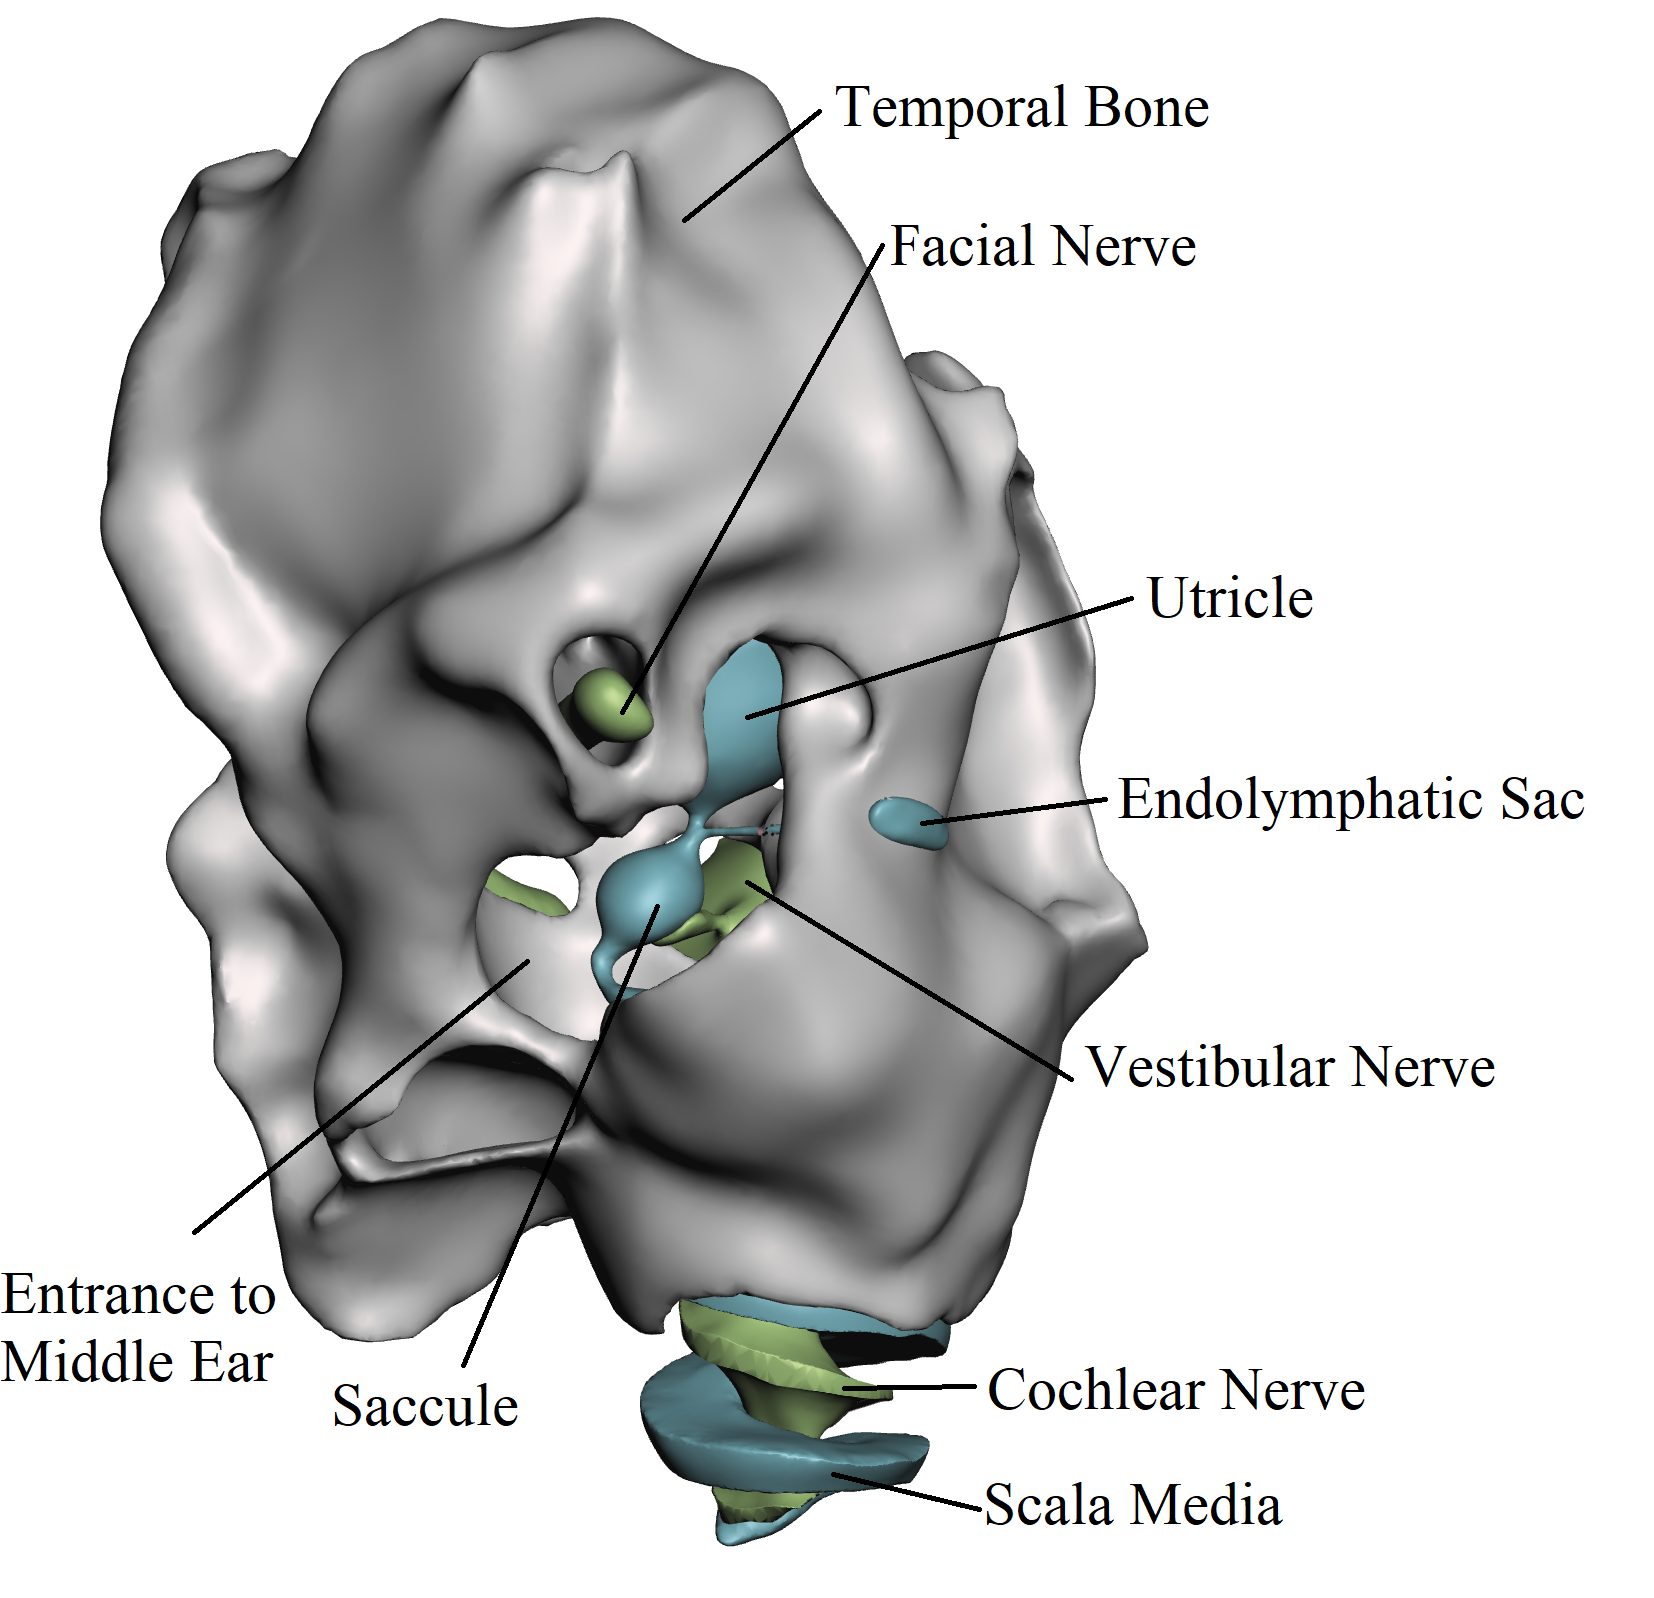
\includegraphics[width=\linewidth]{bonenerve}
	\caption{Bone is shown in white, nerve in green, and the membranous labyrinth in blue}
	\label{bonenerve}
\end{figure}

\begin{figure}[H]
	\centering
	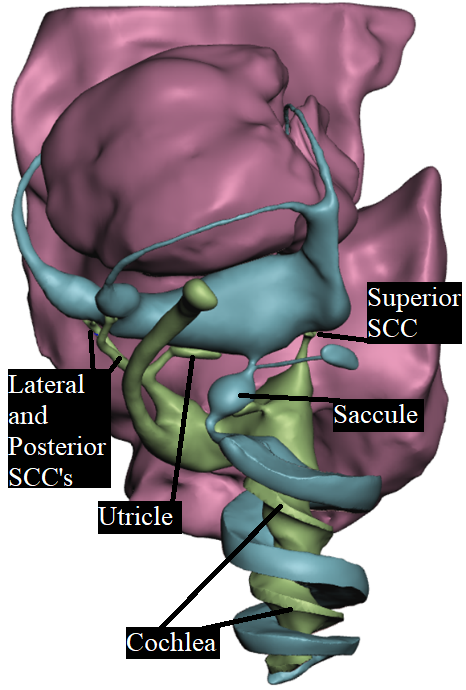
\includegraphics[height=3in]{nervous}
	\caption{Nerves are shown in green and labels are placed at all major attachments of the vestibulocochlear nerve to the membranous labyrinth}
	\label{nvs}
\end{figure}

\begin{figure}[H]
	\centering
	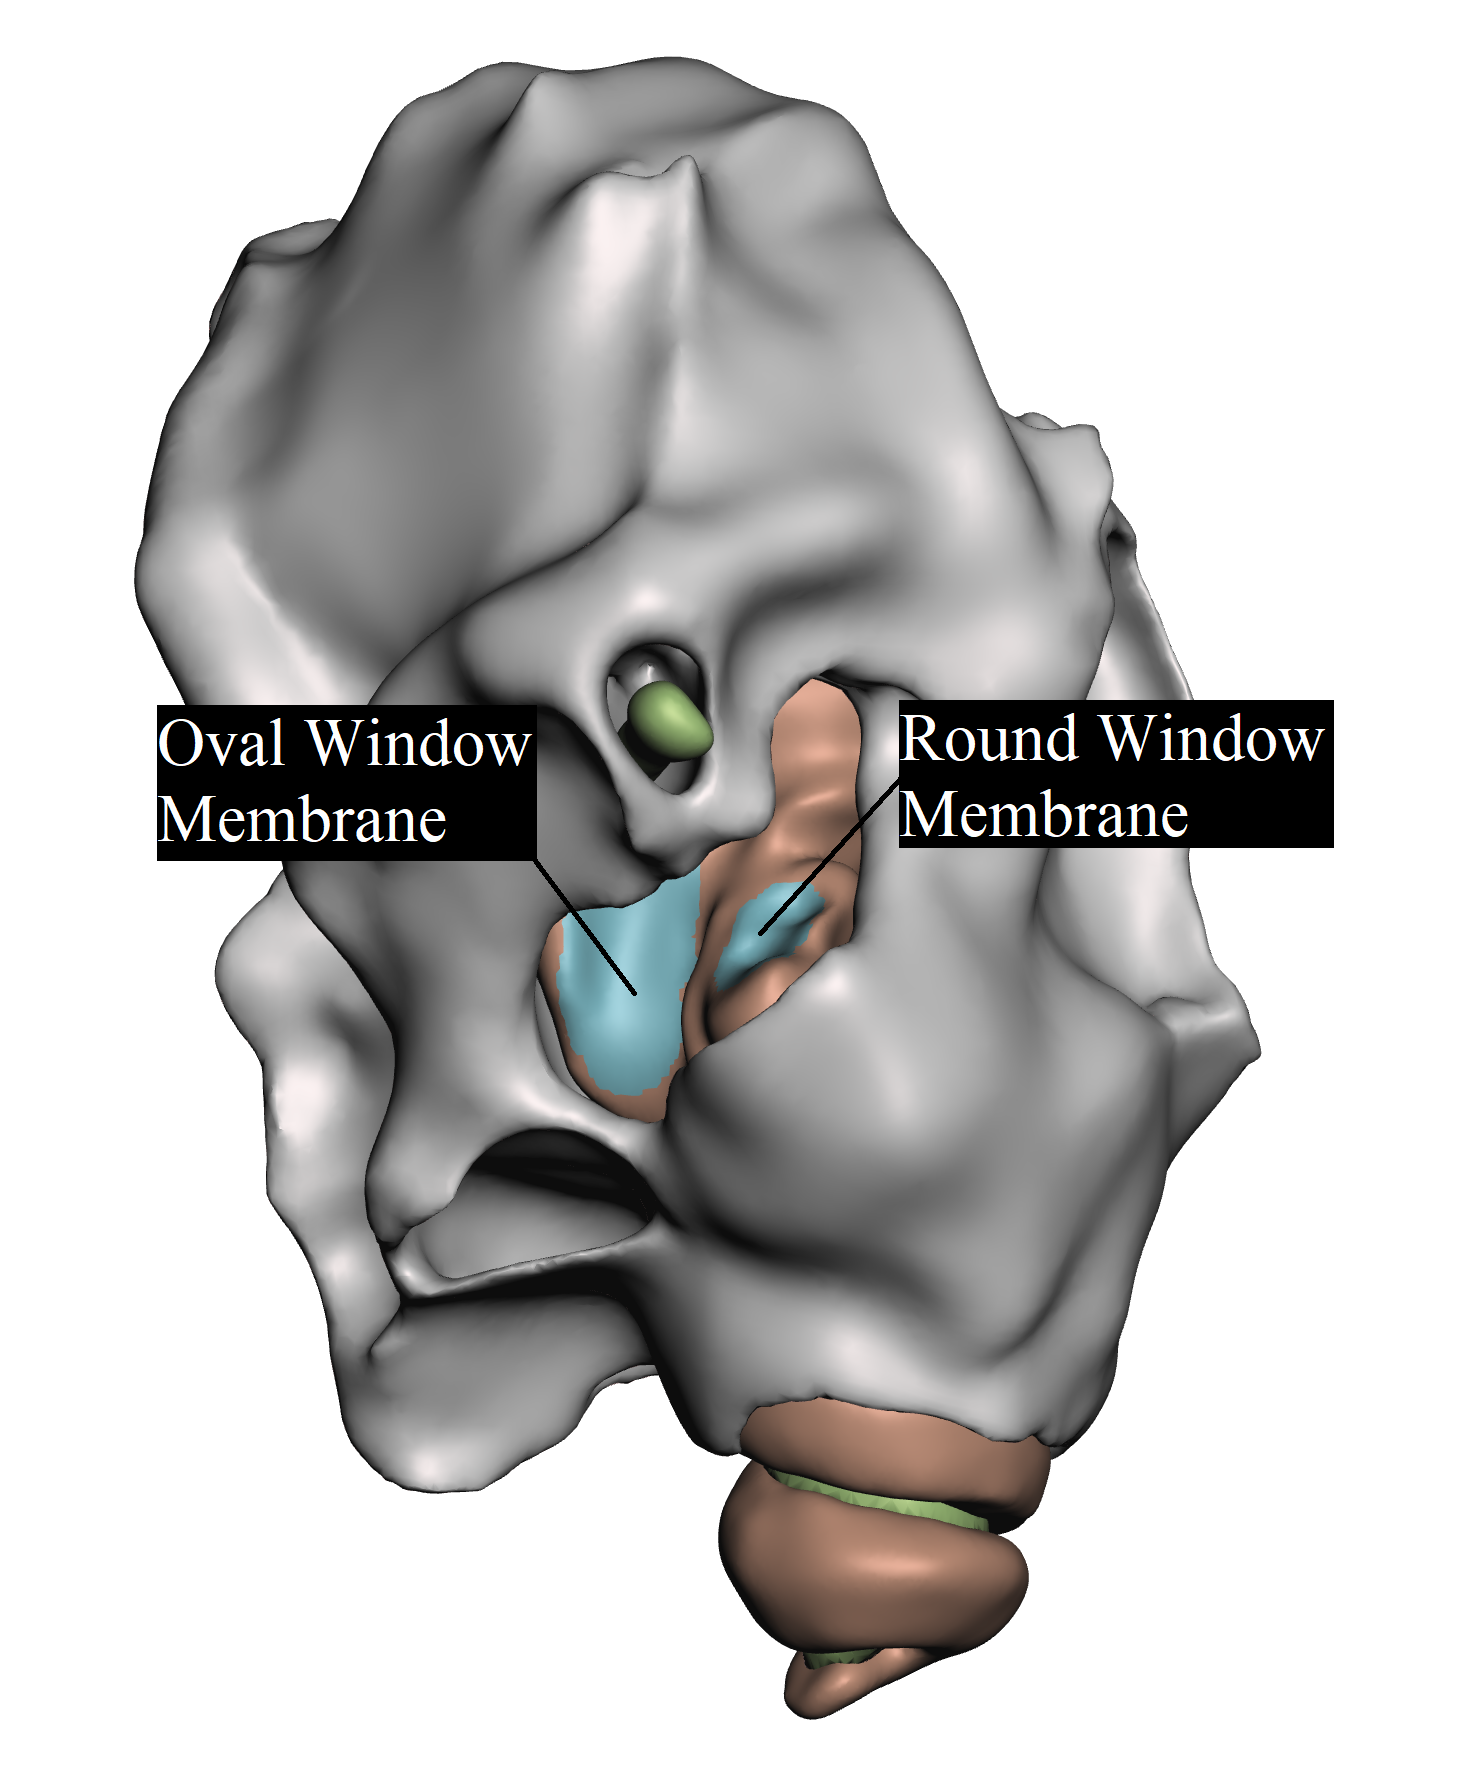
\includegraphics[width=\linewidth]{wm}
	\caption{The round and oval window membranes are denoted in teal on the orange bony labyrinth through the passage from the middle ear in the white temporal bone}
	\label{wm}
\end{figure}

\begin{figure}[H]
\centering
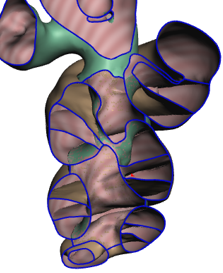
\includegraphics[height=3in]{cochleacx}
\caption{ccx}
\label{ccx}
\end{figure} 

\end{document}